\documentclass[a4paper, titlepage]{article}
\usepackage{xunicode}
\usepackage{fontspec}
\usepackage[frenchb]{babel}
\usepackage{graphicx}
\renewcommand{\familydefault}{\sfdefault}

\renewcommand{\nobreakspace}{\nobreak\ }

\title{Projet HADL: Conception et réalisation}
\author{Julien Durillon \and Alexandre Garnier}
\date{\today}

\begin{document}

	\maketitle

	\tableofcontents\clearpage
	
	\section*{Introduction}
	\addcontentsline{toc}{section}{Introduction}

	  Dans le cadre du module de Composants, nous avons eu à développer une
	  solution logicielle permettant une représentation et une gestion efficaces
	  d'une architecture à composants; ce depuis l'exécution d'une application
	  basée sur l'architecture proposée jusqu'à la méta-méta-modélisation de la
	  solution apportée, c'est à dire la modélisation du paradigme
	  \emph{composant}.

    Dans ce cadre, nous nous sommes intéressés à l'implémentation à base de
    composants d'une architecture Client-Serveur.
    
    Nous avons dès lors choisi de suivre une approche descendante
    (\emph{top-down}) du travail à effectuer. C'est à dire que nous sommes
    partis des concepts permettant la gestion des composants de manière
    générale, pour ensuite les utiliser afin de parvenir à l'implémentation de
    l'application Client-Serveur à proprement parler.

	\section{Niveau M2}
		\subsection{Conception}
			Ce niveau décrit l'architecture d'un système à composants.
		
			%Diagramme général M2
			\begin{figure}[ht]
				\centering
				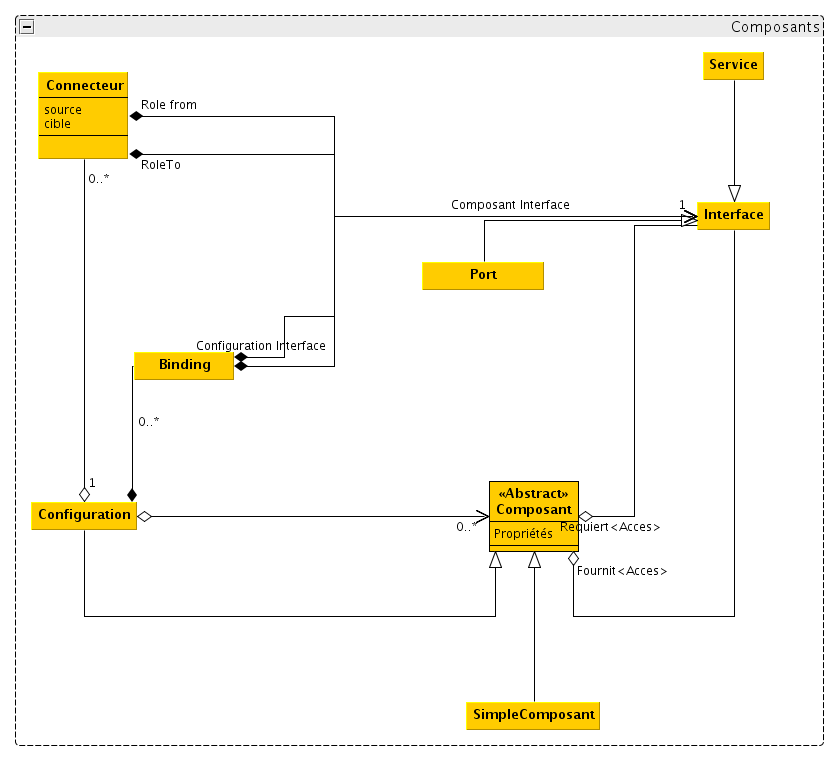
\includegraphics[width=1.00\textwidth]{M2.png}
				\caption{M2: Modèle de l'architecture à composant}
				\label{fig:m2}
			\end{figure}

			La figure \ref{fig:m2} exprime les différents éléments de l'architecture à
			composants et leurs liens.
		
			\paragraph{Composant}
			
				Cette classe est abstraite et doit permettre à n'importe quelle
				classe de se déclarer comme composant en l'étendant.
				
			\paragraph{SimpleComposant et Configuration}
			
				Ces deux classes --- avec Composant--- permettent de fournir un
				pattern composite, demandé par la spécification. Configuration
				est l'objet composite.
			
			\paragraph{Interface}
			
				Un Composant possède des interfaces, qui sont de deux types: Port et
				Service. Ces interfaces sont soit fournies soit requises. Voir page
				\pageref{def:reqfour} pour les interfaces fournies et requises.
				
				
			\paragraph{Connecteur}
			
				Un connecteur connecte une interface fournie (roleFrom) d'un
				composant, et une interface requise (roleTo) d'un autre. Les
				interfaces doivent être de différents composants.
				
				Les connecteurs sont définis dans les configurations. Ils ne
				connectent que les interfaces des composants contenus par la
				configuration.
				
			\paragraph{Binding}
			
				Un Binding fonctionne comme un connecteur, à la différence qu'il
				connecte une interface d'une configuration à une interface d'un de
				ses composants. Les deux interfaces connectées doivent être toutes
				les deux fournies ou requises.
				
				L'appel d'une interface requise d'une configuration doit être passé
				à l'interface requise du composant connecté.
				
				La mise à disposition d'une interface fournie d'un composant doit
				donner lieu à la mise à disposition de l'interface fournie de sa
				configuration associée.
				
			\paragraph{Requise vs fournie}
				\label{def:reqfour}
				Une interface requise est une interface par laquelle on va pouvoir
				passer des messages à un composant. Son nom vient du fait qu'elle va
				requérir des informations.
				
				Une interface requise est une interface qui va fournir des
				informations.
				
				Quand une interface requise est connectée à une interface fournie,
				le connecteur se déclenchera quand l'interface fournies se déclarera
				prête à envoyer des informations.
				
			
			
		\subsection{Implémentation}
		
		Au niveau de l'implémentation, certaines notions ne se présentent plus de
		la même façon:
		
		\subsubsection{Interfaces}
		
			Les interfaces des composants ne sont pas des objets à part, mais sont
			les méthodes et les attributs (resp. service et port) de l'objet
			représentant un composant.
			
		\subsubsection{Composant et Configuration}
		
			Nous avons implémenté les composants comme explicité sur le diagramme.
			Ainsi, nous avons implémenté un pattern composite.
			
			Notre but était de mettre un maximum du code traitant des envois de
			message dans l'implémentation du M2. Ainsi, le M1 ne contiendra que le
			code spécifique.
			
			Pour les messages, nous avons utilisé le pattern Observer-Observable
			comme fournit par java. Les figures \ref{fig:obsimpl} et
			\ref{fig:obsimpl2} décrivent l'architecture
			d'une configuration ainsi que son fonctionnement.
			
			\begin{figure}[ht]
				\centering
				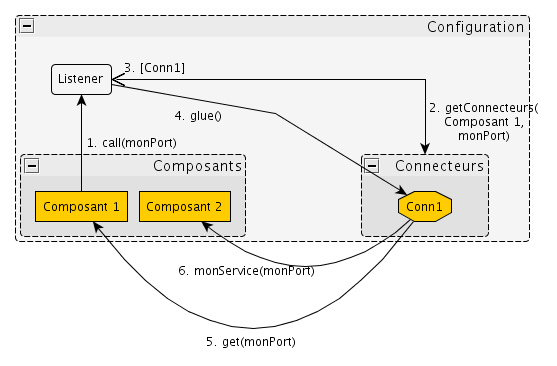
\includegraphics[width=1.00\textwidth]{obsimpl.png}
				\caption{Architecture et fonctionnement d'une configuration: les
				          connecteurs}
				\label{fig:obsimpl}
			\end{figure}
			
			\begin{figure}[ht]
				\centering
				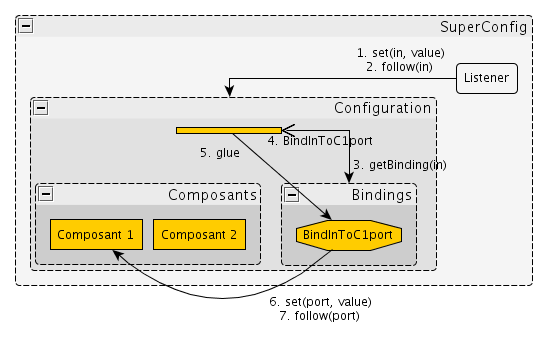
\includegraphics[width=1.00\textwidth]{obsimpl2.png}
				\caption{Architecture et fonctionnement d'une configuration: les
          			  bindings}
				\label{fig:obsimpl2}
			\end{figure}
			
			
	\section{Conception et implémentation du M1 : système client-serveur}
	
	  L'implémentation des concepts liés à la gestion des composants ayant été
	  assurée au niveau M2, l'implémentation propre du système Client-Serveur est
	  dès lors rendue bien plus aisée.
	  
    Ainsi, et dans l'optique de séparer composants et architecture du système,
    nous avons choisi de disposer d'un pool de composants et de connecteurs
    d'une part, et d'un fichier \emph{architecture.xml} décrivant les liens au
    sein de cette architecture d'autre part.
    
    \subsection{Gestion et définition des composants et connecteurs}
    
      
    
    \subsection{Fichier \emph{architecture.xml}}
    
      
	
	\section{Le framework, ou comment tout faire fonctionner}
	
	
	\section{Modélisation de l'architecture à composant}
	
	
	
	
\end{document}
